%NOTE: COMPILE IN TERMINAL USING LUALATEX
\documentclass[a4paper,11pt]{standalone}

\usepackage{tikz-feynman}
%\usetikzlibrary{external}             %% Load the `external` library
%\tikzexternalize
%\immediate\write18{mkdir -p pgf-img}
%\tikzexternalize[                     %% Activate externalization
%  system call={                       %% Use lualatex in system call
%    lualatex \tikzexternalcheckshellescape -halt-on-error -interaction=batchmode -jobname="\image" "\texsource" || rm "\image.pdf"
%  },
%]

\begin{document}

%\feynmandiagram [horizontal=a to b] {
%    i1 -- [fermion,edge label=$d$] a -- [fermion,edge label=$\bar{d}$] i2,
%    a -- [scalar,edge label=$h^0$] b,
%    i1 -- [half left,looseness=0.3,opacity=0] i2,
%};
%\qquad
%\feynmandiagram [layered layout, horizontal=a to b] {
%    a -- [fermion,edge label=$b$] b -- [fermion,edge label=$c$] f1, 
%    b -- [scalar,edge label=$H^-$] c,
%    c -- [anti fermion,edge label=$\nu_l$] f2,
%    c -- [fermion,edge label=$l^-$] f3,
%};
%\feynmandiagram [layered layout, horizontal=a to b] {
%    i1 -- [fermion,edge label=$q$] a -- [boson,edge label=$W^-$] b -- [anti fermion,edge label=$\bar{q}$] f1,
%    i2 -- [anti fermion,edge label'=$\bar{b}$] c -- [boson,edge label'=$W^+$] d -- [fermion,edge label'=$b$] f2,
%    {[same layer] a -- [fermion,edge label'=${u,c,t}$] c},
%    {[same layer] b -- [fermion,edge label=${u,c,t}$] d},
%    {[same layer] i1 -- [half left,looseness=0.3] i2},
%    {[same layer] i1 -- [half right,looseness=0.3,edge label'=$B_q^0$] i2},
%    {[same layer] f2 -- [half left,looseness=0.3] f1},
%    {[same layer] f2 -- [half right,looseness=0.3,edge label'=$\bar{B}_q^0$] f1},
%};

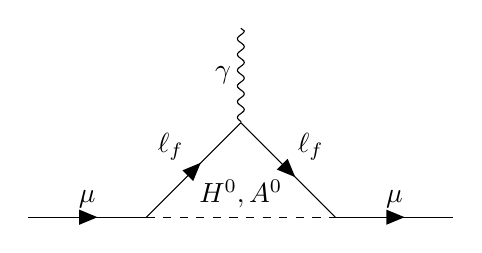
\begin{tikzpicture}
    \begin{feynman}
        \vertex (a1);
        \vertex[right=1.5cm of a1] (a2);
        \vertex[right=1.2cm of a2] (a3);
        \vertex[right=1.2cm of a3] (a4);
        \vertex[right=1.5cm of a4] (a5);
        \vertex[above=1.2cm of a3] (b1);
        \vertex[above=1.2cm of b1] (b2);

        \diagram* {
            (a1) -- [fermion,edge label=$\mu$] (a2) -- [scalar,edge label={$H^0,A^0$}] (a4) -- [fermion,edge label=$\mu$] (a5);
            (a2) -- [fermion,edge label=$\ell_f$] (b1) -- [fermion,edge label=$\ell_f$] (a4);
            (b1) -- [boson,edge label=$\gamma$] (b2);
        };
    \end{feynman}
\end{tikzpicture}
\qquad
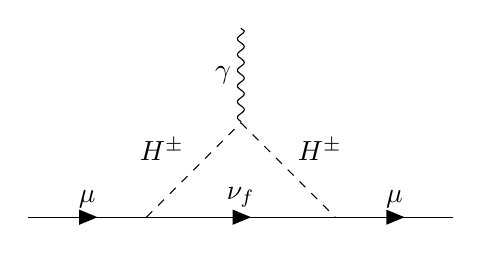
\begin{tikzpicture}
    \begin{feynman}
        \vertex (a1);
        \vertex[right=1.5cm of a1] (a2);
        \vertex[right=1.2cm of a2] (a3);
        \vertex[right=1.2cm of a3] (a4);
        \vertex[right=1.5cm of a4] (a5);
        \vertex[above=1.2cm of a3] (b1);
        \vertex[above=1.2cm of b1] (b2);

        \diagram* {
            (a1) -- [fermion,edge label=$\mu$] (a2) -- [fermion,edge label=$\nu_f$] (a4) -- [fermion,edge label=$\mu$] (a5);
            (a2) -- [scalar,edge label=$H^\pm$] (b1) -- [scalar,edge label=$H^\pm$] (a4);
            (b1) -- [boson,edge label=$\gamma$] (b2);
        };
    \end{feynman}
\end{tikzpicture}

%\begin{tikzpicture}
%    \begin{feynman}
%        \vertex (a1);
%        \vertex[below=3cm of a1] (a2);
%        \vertex[below right=1cm and 1.5cm of a1] (a3);
%        \vertex[below=1cm of a3] (a4);
%        \vertex[above right=0.5cm and 1cm of a4] (a5);
%        \vertex[right=1.5cm of a5] (a6);
%        \vertex[above right=1cm and 1.5cm of a6] (a7);
%        \vertex[below=2cm of a7] (a8);
%
%        \diagram* {
%            (a1) -- [fermion,edge label=$q$] (a3) -- [scalar,edge label'=$H^-$] (a4) -- [fermion,edge label=$\bar{b}$] (a2);
%            (a3) -- [quarter left,fermion,edge label=${u,c,t}$] (a5) -- [quarter left,fermion,edge label=${u,c,t}$] (a4);
%            (a5) -- [scalar,edge label=${h^0,H^0,A^0}$] (a6);
%            (a7) -- [fermion,edge label'=$\mu^+$] (a6) -- [fermion,edge label'=$\mu^-$] (a8);
%            (a1) -- [half left,looseness=0.3] (a2) -- [half left,looseness=0.3,edge label=$B_q$] (a1);
%        };
%    \end{feynman}
%\end{tikzpicture}

\end{document}
